\documentclass[a4paper, foldmark, 12pt]{leaflet}
%\documentclass[a4paper, foldmark, nocombine]{leaflet}
\usepackage[utf8]{inputenc}
\usepackage{color}
\usepackage{hyperref}
\usepackage{times}
\usepackage{floatflt}

%% Example users
\newcommand{\UserI}{\textit{Alice}}
\newcommand{\UserII}{\textit{Ben}}
\newcommand{\UserIII}{\textit{Christine}}

%% Example movies
\newcommand{\MovieI}{\textit{The Usual Suspects}}
\newcommand{\MovieII}{\textit{American Beauty}}
\newcommand{\MovieIII}{\textit{The Godfather}}
\newcommand{\MovieIV}{\textit{Road Trip}}


\usepackage{fancyhdr}

\pagestyle{fancy}

\fancyhead{}
\fancyfoot{}

\renewcommand{\headrulewidth}{0.0pt}
\renewcommand{\footrulewidth}{0.4pt}

\fancyhead[CO,CE]{
	\vspace{-1cm}
	\begin{center}
		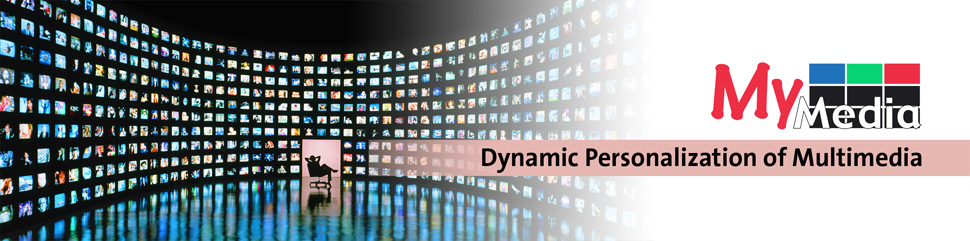
\includegraphics[width=9.0cm]{fig/MyMediaScreenwallBanner.jpg}
	\end{center}	
}
\fancyfoot[C]{\thepage}

%\setmargins{3cm}{2cm}{1cm}{1cm}

\headheight = 2cm



\title{MyMediaLite -- Recommender System Algorithm Library}

\author{
	
\includegraphics[width=4.0cm]{fig/uni-hildesheim-400x400.jpg}\\
	Machine Learning Lab
}
\date{October 2010}

\begin{document}

\maketitle

MyMediaLite is a lightweight, multi-purpose library
of recommender system algorithms.
It addresses the two most common scenarios in collaborative filtering:
rating prediction (e.g. on a scale of 1 to 5 stars)
and item prediction from implicit feedback (e.g. from clicks or purchase actions).

\begin{center}
	\url{http://ismll.de/mymedialite/}
\end{center}

\newpage

\section{MyMediaLite's Key Features}

\begin{itemize}
	\item \textbf{Choice:}
		\begin{itemize}
			\item Dozens of different recommender engines (see list on this flyer),
			\item methods can use collaborative and attribute/content data.
		\end{itemize}
	\item \textbf{Serialization:} save and reload recommender engine models.
	\item \textbf{Real-time online updates} for most models.
	\item \textbf{Ready to use:}
		\begin{itemize}
			\item Includes evaluation routines for rating and item prediction;
			      quality measures MAE, RMSE, AUC, prec@N, MAP, NDCG; and
			\item command line tools that read a simple text-based input format.
		\end{itemize}
	\item \textbf{Compact:} Core library is 85KB ``big''.
	\item \textbf{Portable:} Written in C\#, for the .NET platform;
	      runs on every architecture where \href{www.mono-project.com}{Mono} works:
	      Linux, Windows, Mac OS X.
	\item \textbf{Free:} Free/Open Source software, distributed under the terms of the
	      GNU General Public License (GPL).
\end{itemize}

\newpage

\section{Target Groups}

\subsection{Researchers}
\begin{itemize}
	\item Don't waste your time implementing methods
	      if you actually want to study
	      other aspects of recommender systems!
	\item Use the engines as baseline methods in benchmarks.
	\item Use MyMediaLite's infrastructure as an easy
	      starting point to implement your own methods.
\end{itemize}

\subsection{Developers}
\begin{itemize}
	\item Add recommender system technologies to your software.
\end{itemize}

\subsection{Students}
\begin{itemize}
	\item See how typical recommender system methods are implement.
	\item Use MyMediaLite as a basis for you school projects.
\end{itemize}

\newpage

\section{Recommendation Tasks Addressed}

\subsection{Rating Prediction}

Popularized by systems like MovieLens, Netflix, or Jester,
this is the most-discussed collaborative filtering task in the
recommender systems literature.
Given a set of ratings, e.g. on a scale from 1 to 5,
the goal is predict unknown ratings.

\begin{center}
      \begin{tabular}{|l||c|c|c|}
        \hline
	           & \UserI & \UserII & \UserIII \\ \hline
	\hline
	\MovieI    &  5   &     & 4     \\ \hline
	\MovieII   &  3   & 4   & 3    \\ \hline
	\MovieIII  &      & \textbf{??}    & 1    \\ \hline
	\MovieIV   &  2   &     &        \\ \hline
      \end{tabular}
\end{center}


\subsection{Implicit Feedback Item Recommendation}

Getting ratings from users requires explicit actions from their side.
Much more data is available in the form of implicit feedback,
e.g. whether a user has viewed or purchased a product in an online shop.
Very often this information is positive-only,
i.e. we know users like the products they buy, but we cannot easily assume
that they do not like everything they have not (yet) bought.

\begin{center}
	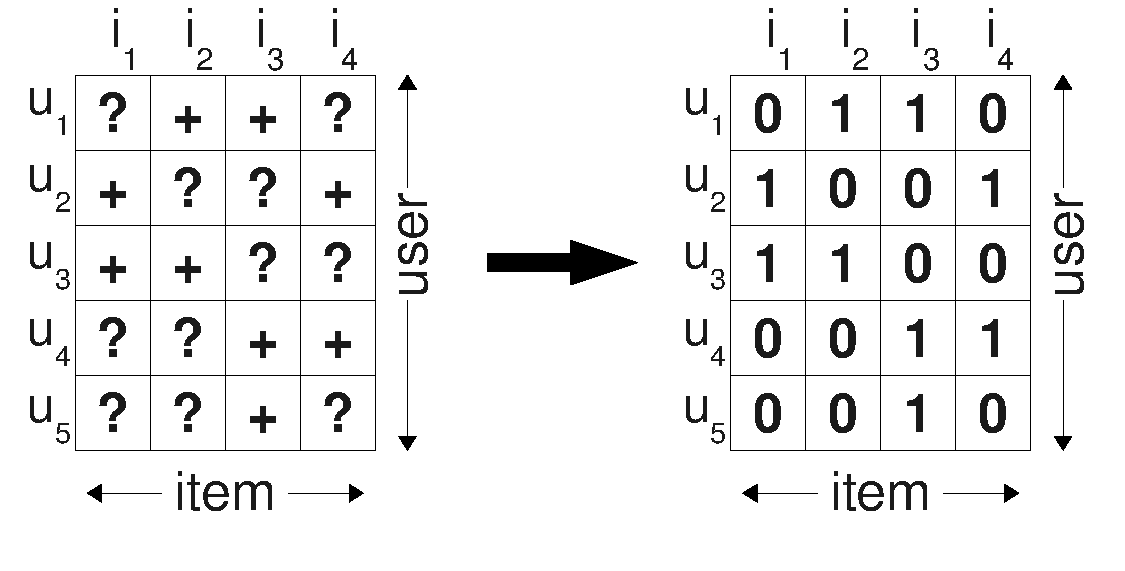
\includegraphics[width=7.0cm]{fig/interpretation_single.pdf}
\end{center}

\newpage 

\section{Implemented Methods}
Rating Prediction
\begin{itemize}
	\item averages: global, user, item
	\item linear baseline method by Koren and Bell
	\item k-nearest neighbor (kNN):
		\begin{itemize}
			\item based on user or item similarities
			\item collaborative or attribute-/content-based
			\item different similarity measures: Pearson correlation, Cosine similarity
		\end{itemize}
	\item (biased) matrix factorization
\end{itemize}

Item Prediction
\begin{itemize}
	\item random
	\item most popular Iiem
	\item linear content-based model optimized for Bayesian Personalized Ranking (BPR-Linear)
	\item k-nearest neighbor (kNN):
		\begin{itemize}
			\item based on user or item similarities
			\item collaborative or attribute-/content-based
		\end{itemize}
	\item weighted regularized matrix factorization (WR-MF)
	\item matrix factorization optimized for Bayesian Personalized Ranking (BPR-MF)
\end{itemize}

\newpage

\section{Download}
Get the latest release of MyMediaLite here:
\begin{center}
	\url{http://ismll.de/mymedialite/}
\end{center}

\section{Contact}
We would like to get feedback (suggestions, bug reports, etc.) about MyMediaLite.
To contact us, send an e-mail to
\begin{center}
	\texttt{mymedialite@ismll.de}
\end{center}

\section{Acknowledgements}

\begin{floatingfigure}[r]{1.6cm}
	\vspace{-0.5cm}
	
\includegraphics[width=2.1cm]{fig/uni-hildesheim-400x400.jpg}
\end{floatingfigure}
MyMediaLite was developed by Zeno Gantner,
Steffen Rendle, and Christoph Freudenthaler
at University of Hildesheim.
	
\vspace{0.4cm}

This work was partly funded by the European Commission FP7 project MyMedia
(Dynamic Personalization of Multimedia, \url{http://www.mymediaproject.org/})
under the grant agreement no. 215006.

\vspace{0.2cm}

\begin{center}
	
\includegraphics[width=4.0cm]{fig/MyMediaLogoMedium.png}
	\hspace{1.5cm}
	
\includegraphics[width=2.0cm]{fig/logo-fp7.png}\\
\end{center}

\end{document}
